\documentclass[12pt, letterpaper, twoside]{article}
\usepackage[utf8]{inputenc}
\usepackage{geometry}
\usepackage{graphicx}
\usepackage{amsmath,amssymb}
\usepackage{enumitem}
\usepackage{physics}
\usepackage{xcolor}
\usepackage{multicol}
\setlength{\columnsep}{1cm}
\newcommand\numberthis{\addtocounter{equation}{1}\tag{\theequation}}
\geometry{a4paper, total={160mm,250mm}, left=25mm, top=20mm}
\title{Quadratic NLS Simulations}
\author{Realeboga Dikole}

\begin{document}

\maketitle

\section{Numerical Solution of the Quadratic NLS}
The equation in question is the quadratic nonlinear Schr\"odinger equation and it states 
\begin{equation}\label{quad-NLS-lambda}
     \left(i + \lambda \right) \frac{\partial \psi}{\partial t} - \frac{\partial^2 \psi}{\partial x^2} - 6 \psi^{2} =  - 4 \psi + b (\psi - \psi^{*}),  
\end{equation}
where $\lambda = 0$ in the simulations below.
 The numerical method used here is the Fourier spectral differentiation method, where we take $\mathcal{D}_{N}^{(2)}$ as an approximation of spatial derivatives, with the superscript of $2$ denoting the order of the derivative and subscript denotes that the matrix is $N \times N$. The time derivatives are approximated using the centered differences as follows 
 \begin{equation}
     \frac{\partial \psi(x, t)}{\partial t} \approx \frac{\psi_{j}^{n+1} - \psi_{j}^{n-1}}{2 \tau} + \mathcal{O}(\tau^{2}), 
 \end{equation}. 
where we have defined $\psi(x, t)$ in its discrete form as $\psi(x_j, t_n) = \psi_{j}^{n} $
For approximating the satial part of $\psi(x, t)$ we make use of  differentiation matrix $\mathcal{D}_{N}^{(2)}$ which is given by the following 
\begin{equation}
\mathcal{D}_{N}^{(2)} = 
    \begin{pmatrix}
     & \qquad \vdots  \qquad& \\
     \ddots & \qquad -\frac{1}{2}\csc^{2}\left( \frac{2h}{2}\right) \qquad & \\
     \ddots &  \qquad  \frac{1}{2}\csc^2 \left( \frac{h}{2}\right) \qquad &\\
    \ddots & \qquad   - \frac{\pi^2}{3h^2} - \frac{1}{6}  \\
     & \qquad  \frac{1}{2}\csc^2\left( \frac{h}{2}\right) & \qquad \ddots \\
     & \qquad  - \frac{1}{2}\csc^2\left( \frac{2h}{2}\right) &\qquad  \ddots\\ \\
     
     & \qquad \vdots \qquad & \ddots&
    \end{pmatrix}.
\end{equation}
\newline
The matrix $\mathcal{D}_{N}^{(2)}$ is an operator and it acts on $\psi_{j}^{2}$ at each time step $\tau$ to approximate the derivative at the particular time step.
The discrete form of \eqref{quad-NLS} reads
\begin{equation}\label{discrete-quad-NLS}
    \psi_{j}^{n+1} = \psi_{j}^{n-1}  + \left(\frac{2 \tau}{i + \lambda}\right) \left\lbrace \frac{\pi^2}{L^2} \mathcal{D}^{(2)}_{N} \psi^{n}_{j} + 6 (\psi^{n}_{j})^2 - 4 \psi^{n}_{j} + b \left(\psi_{j}^{n} - (\psi_{j}^{n})^{*} \right) \right\rbrace, 
\end{equation}

 See the plots below for the simulations of \eqref{quad-NLS} --- a stationary solution known as the \textit{fundamental soliton/ sech mode } is considered as an initial condition when $b=0$ and $\lambda = 0$. The \textit{fundamental soliton} reads
\begin{equation}\label{sech-mode}
    u_s(x) = \sech^{2}(x), 
\end{equation}
where the subscript $s$ denotes the fact that this is a stationary solution.
 The simulation is done on the interval $[-20\pi, 20\pi]$ and only the interval $[-2\pi, 2\pi]$ is shown for better viewing. The time variable $t$ runs on the interval $[0, 50]$.

 \begin{enumerate}[label=(\roman*)]
\item \textbf{Solution for $b = 0$, $\lambda = 0$:}
\begin{multicols}{2}
    \begin{center}
        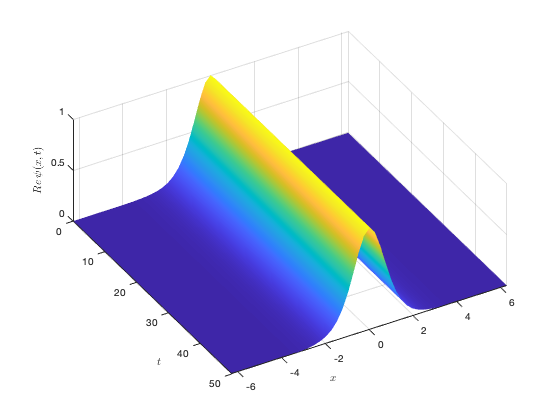
\includegraphics[scale=0.4]{Figures/b0real.png}
    \end{center}
    
    \begin{center}
        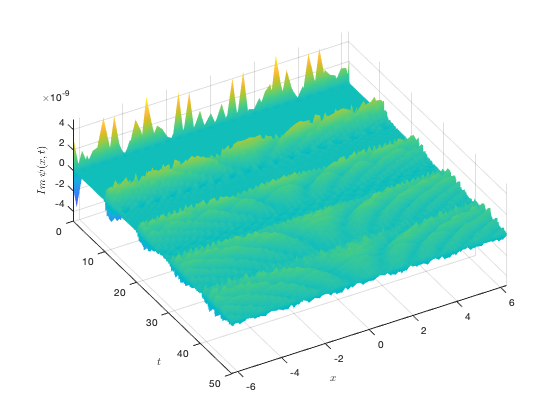
\includegraphics[scale=0.4]{Figures/b0imag.png}
    \end{center}
\end{multicols}
\figurename{ 1.1 The Fourier spectral solution of the quadratic NLS. The real part solution is on the left, and the imaginary part of the  solution if on the right. }

\end{enumerate}

\section{Fundamental soliton and its instability}

 To investigate the stability of \eqref{sech-mode} we add a small perturbation and evolve it according to \eqref{quad-NLS-lambda}. The choice of our perturbation is $\epsilon \cos(x)$, where $\epsilon$ is small enough to ensure the solutions don't blow up completely. The new intial conditions now reads
 \begin{equation}\label{sech-perturbation}
     u(x) = u_s(x) + \epsilon \cos(x)
 \end{equation}
 

\subsection{Numerical results}
All the simulations below were performed without the inclusion of the friction term $\lambda \partial_t \psi$ in \eqref{quad-NLS}. See the plots below.

\begin{enumerate}[label=(\roman*)]
\item \textbf{Solution for $b = -3$, $\lambda=0$ and $\epsilon = 10^{-13}$:}
\begin{multicols}{2}
\begin{center}
    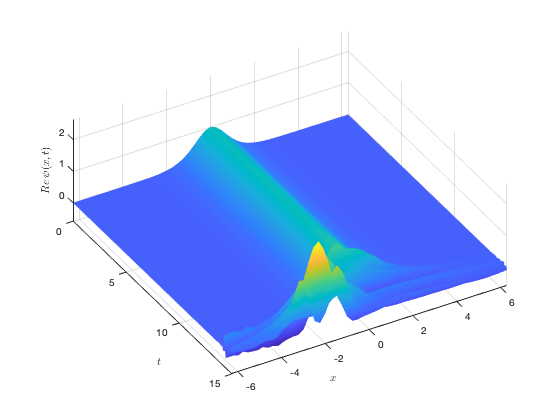
\includegraphics[scale=0.35]{Figures/(b-3real).png}
\end{center}
\begin{center}
    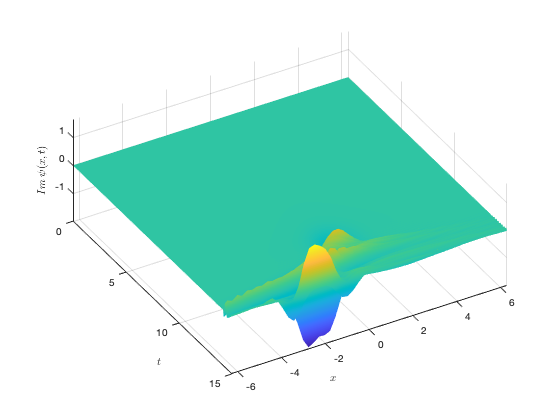
\includegraphics[scale=0.35]{Figures/(b-3imag).png}
\end{center}
\end{multicols}
\figurename{ 2.1.1 (a) The real (left) and imaginary (right) parts of $\psi(x, t)$}


\begin{center}
    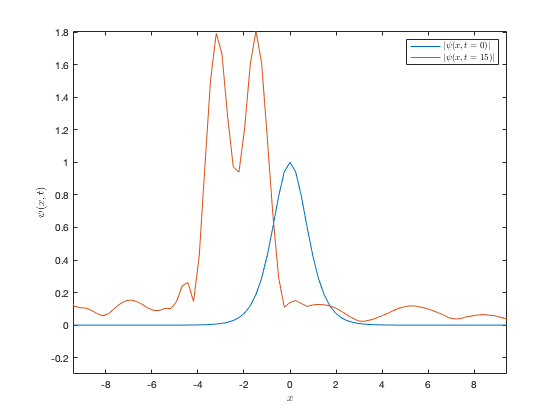
\includegraphics[scale=0.5]{Figures/soliton disintegration b minus 3.png}
\end{center}
\figurename{ 2.1.1 (b)The graph of $|\psi(x,t)|$ at showing the initial condition (blue) at time $t = 0$ and the disintegration of the initial wave form at time $t = 15$. }
\item \textbf{Solution for $b = -2$, $\lambda=0$ and $\epsilon = 10^{-3}$:}
\begin{multicols}{2}
\begin{center}
    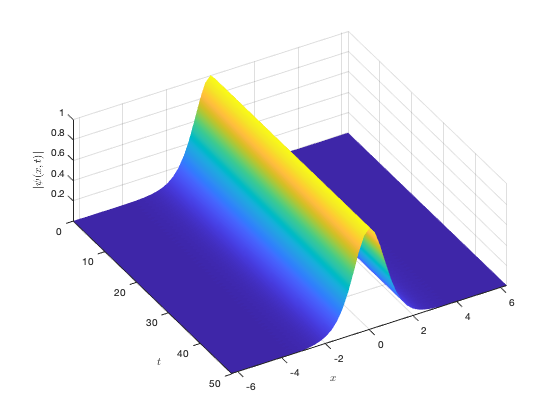
\includegraphics[scale=0.35]{Figures/(b-2real).png}
\end{center}
\begin{center}
    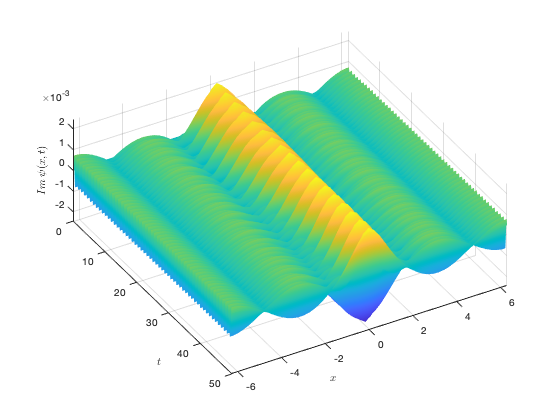
\includegraphics[scale=0.35]{Figures/(b-2imag).png}
\end{center}
\end{multicols}
\figurename{ 2.1.2 The real (left) and imaginary (right) parts of $\psi(x, t)$}

\item \textbf{Solution for $b = -1$, $\lambda=0$ and $\epsilon = 10^{-3}$:}
\begin{multicols}{2}
\begin{center}
    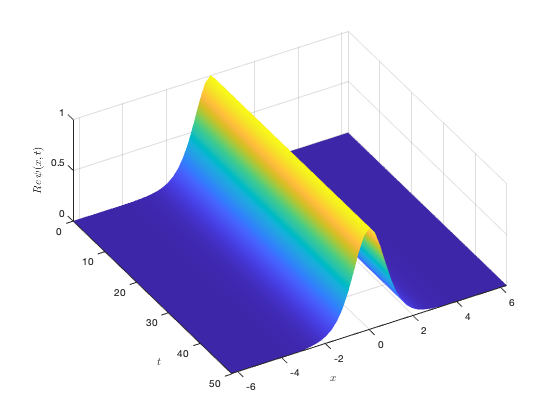
\includegraphics[scale=0.35]{Figures/(b-1real).png}
\end{center}
\begin{center}
    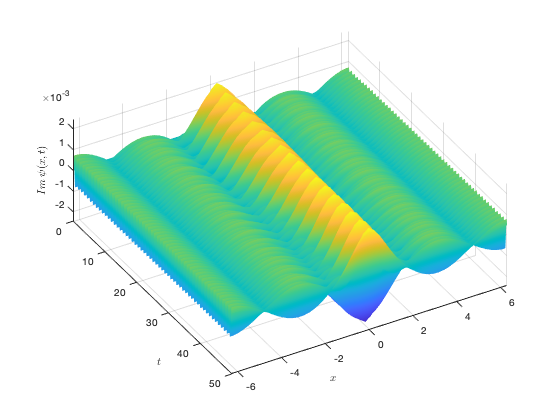
\includegraphics[scale=0.35]{Figures/(b-1imag).png}
\end{center}
\end{multicols}
\figurename{ 2.1.3 The real (left) and imaginary (right) parts of $\psi(x, t)$}

\item \textbf{Solution for $b = 0$, $\lambda=0$ and $\epsilon = 10^{-3}$:}
\begin{multicols}{2}
\begin{center}
    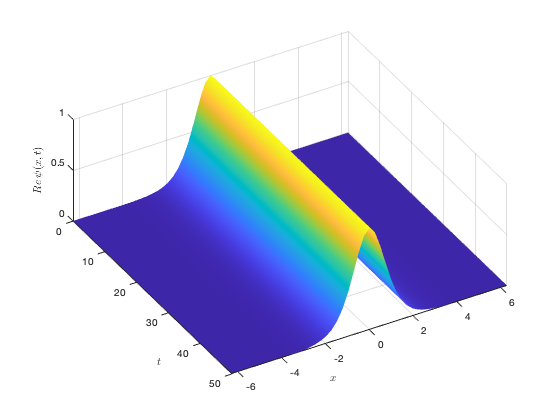
\includegraphics[scale=0.35]{Figures/(b0real).png}
\end{center}
\begin{center}
    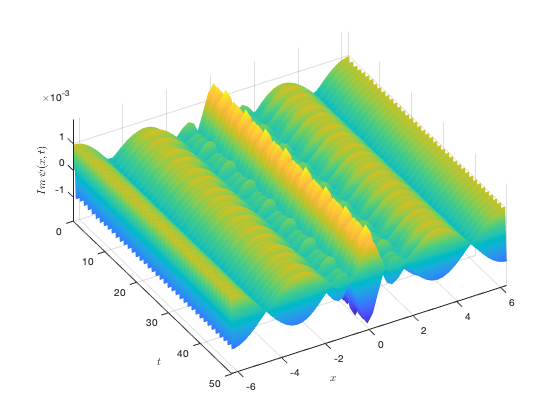
\includegraphics[scale=0.35]{Figures/(b0imag).png}
\end{center}
\end{multicols}
\figurename{ 2.1.4 The real (left) and imaginary (right) parts of $\psi(x, t)$}

\item \textbf{Solution for $b = 1$, $\lambda=0$ and $\epsilon = 10^{-3}$:}
\begin{multicols}{2}
\begin{center}
    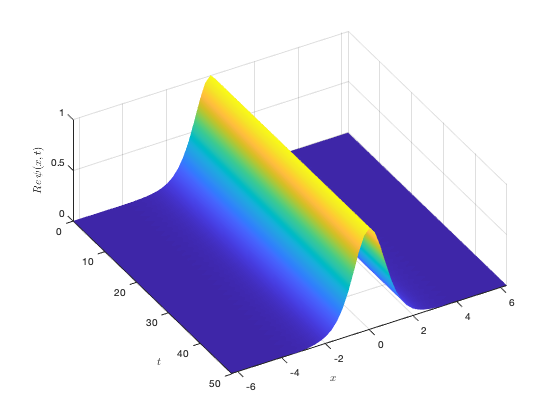
\includegraphics[scale=0.35]{Figures/(b1real).png}
\end{center}
\begin{center}
    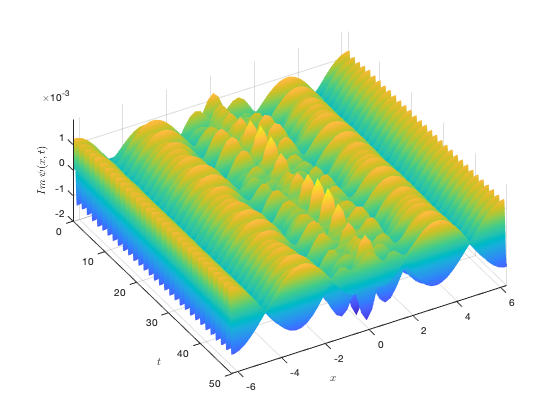
\includegraphics[scale=0.35]{Figures/(b1imag).png}
\end{center}
\end{multicols}
\figurename{ 2.1.5 The real (left) and imaginary (right) parts of $\psi(x, t)$}


\item \textbf{Solution for $b = 2$, $\lambda=0$ and $\epsilon = 10^{-13}$:}
\begin{multicols}{2}
\begin{center}
    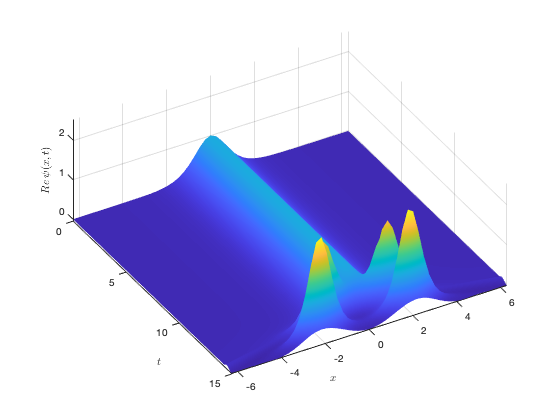
\includegraphics[scale=0.35]{Figures/(b2real).png}
\end{center}
\begin{center}
    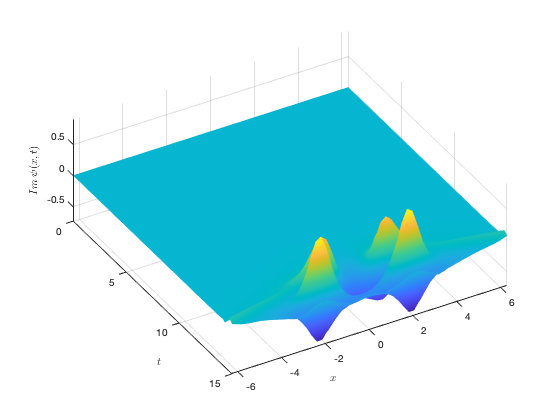
\includegraphics[scale=0.35]{Figures/(b2imag).png}
\end{center}
\end{multicols}
\figurename{ 2.1.6 (a) The real (left) and imaginary (right) parts of $\psi(x, t)$}

\begin{center}
    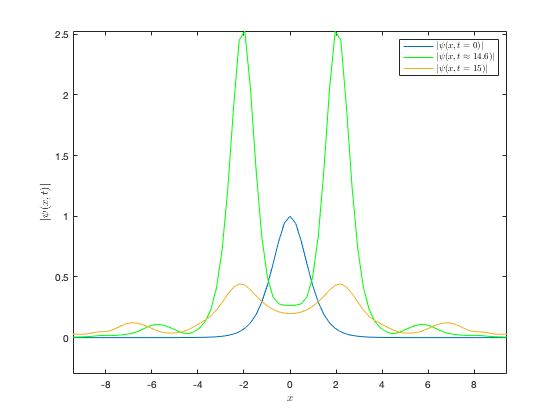
\includegraphics[scale=0.5]{Figures/b2 soliton disintegration.png}
\end{center}
\figurename{ 2.1.6 (b)The graph of $|\psi(x,t)|$ at showing the initial condition (blue) at time $t = 0$ and the disintegration of the initial wave form (green) at time $t \approx 14.6$, where the soliton jumps to maximum $|\psi| = 2.5$ and then drops lower (orange) than $|\psi| = 0.5$ at $t = 15$. }

\end{enumerate}


\section{Inclusion of the damping coefficient}

We have previously shown the numerical simulations of \eqref{quad-NLS-lambda} and its instability in the absence of the friction term. Now we consider the same perturbed initial condition \eqref{sech-perturbation} for the nonzero friction coefficient $\lambda$. See plots bellow.

\begin{enumerate}[label=(\roman*)]
    \item \textbf{Solution for $b=-3$, $\lambda=0.3$ and $\epsilon=10^{-5}$:}
    
    \begin{multicols}{2}
        \begin{center}
            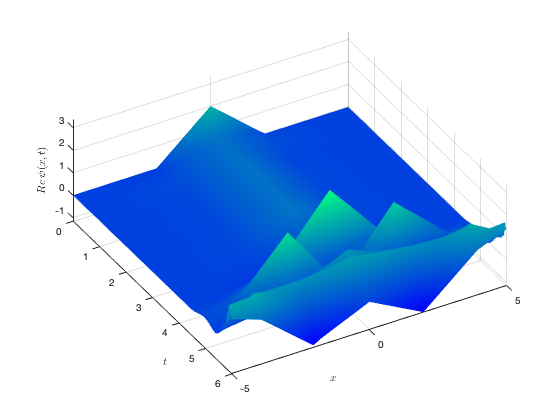
\includegraphics[scale=0.35]{with friction/(b-3real).png}
        \end{center} 
        \begin{center}
            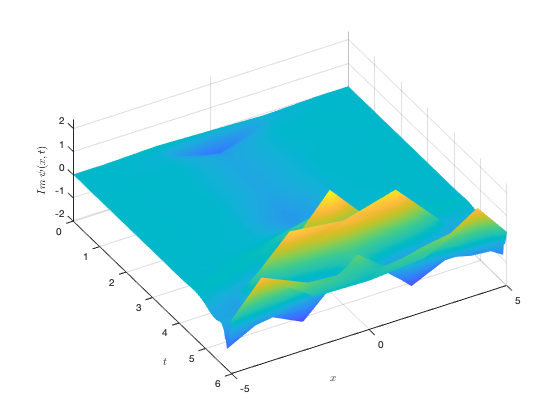
\includegraphics[scale=0.35]{with friction/(b-3imag).png}
        \end{center}  
    \end{multicols}
    \figurename{ 3.1 The real (left) and imaginary (right) parts of $\psi(x, t)$}
    \newpage
    \item \textbf{Solution for $b=-2$, $\lambda=0.3$ and $\epsilon=10^{-5}$:}
    
    \begin{multicols}{2}
        \begin{center}
            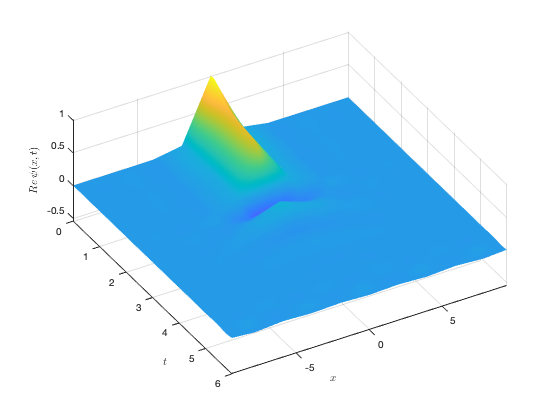
\includegraphics[scale=0.35]{with friction/(b-2real).png}
        \end{center} 
        \begin{center}
            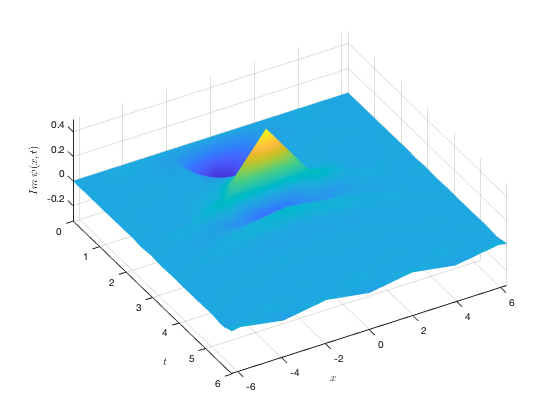
\includegraphics[scale=0.35]{with friction/(b-2imag).png}
        \end{center}  
    \end{multicols}
    \figurename{ 3.2 The real (left) and imaginary (right) parts of $\psi(x, t)$}
    
    \item \textbf{Solution for $b=-1$, $\lambda=0.3$ and $\epsilon=10^{-5}$:}
    \begin{multicols}{2}
        \begin{center}
            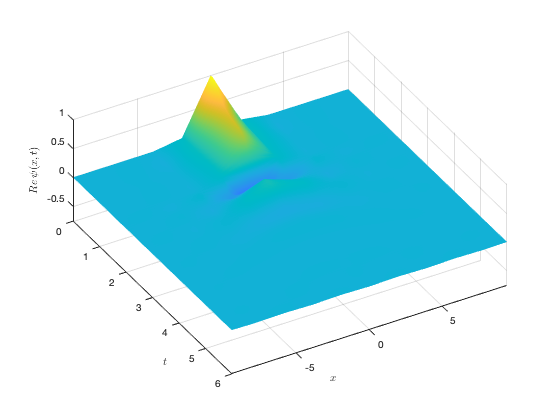
\includegraphics[scale=0.35]{with friction/(b-1real).png}
        \end{center} 
        \begin{center}
            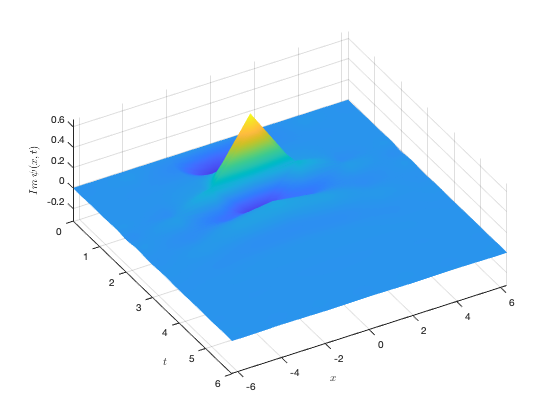
\includegraphics[scale=0.35]{with friction/(b-1imag).png}
        \end{center}  
    \end{multicols}
    \figurename{ 3.3 The real (left) and imaginary (right) parts of $\psi(x, t)$}
    
    \item \textbf{Solution for $b=0$, $\lambda=0.3$ and $\epsilon=10^{-5}$:}
   \begin{multicols}{2}
        \begin{center}
            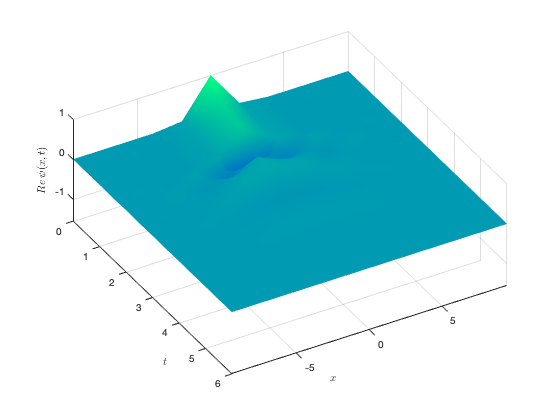
\includegraphics[scale=0.35]{with friction/b0real.png}
        \end{center} 
        \begin{center}
            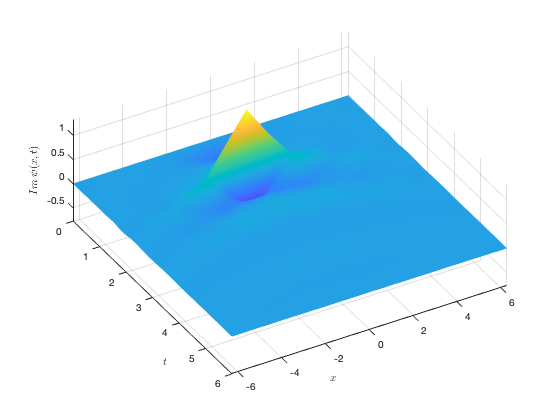
\includegraphics[scale=0.35]{with friction/b0imag.png}
        \end{center}  
    \end{multicols}
    \figurename{ 3.4 The real (left) and imaginary (right) parts of $\psi(x, t)$}
    \newpage
    
    \item \textbf{Solution for $b=1$, $\lambda=0.3$ and $\epsilon=10^{-5}$:}
   \begin{multicols}{2}
        \begin{center}
            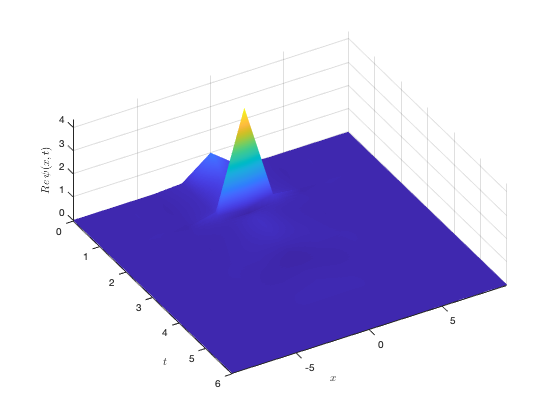
\includegraphics[scale=0.35]{with friction/b1real.png}
        \end{center} 
        \begin{center}
            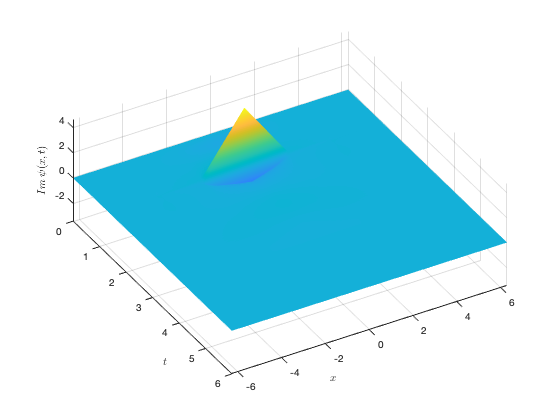
\includegraphics[scale=0.35]{with friction/b1imag.png}
        \end{center}  
    \end{multicols}
    \figurename{ 3.5 The real (left) and imaginary (right) parts of $\psi(x, t)$}
    
    \item \textbf{Solution for $b=2$, $\lambda=0.3$ and $\epsilon=10^{-5}$:}
   \begin{multicols}{2}
        \begin{center}
            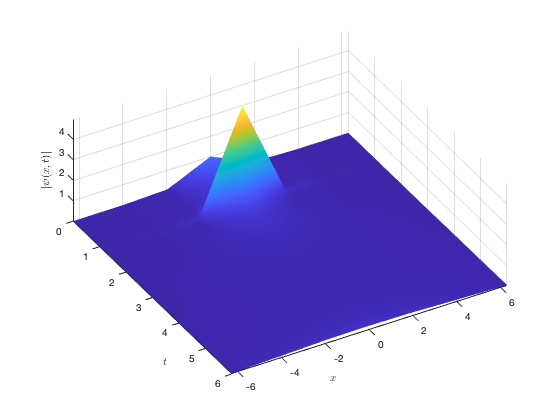
\includegraphics[scale=0.35]{with friction/b2real.png}
        \end{center} 
        \begin{center}
            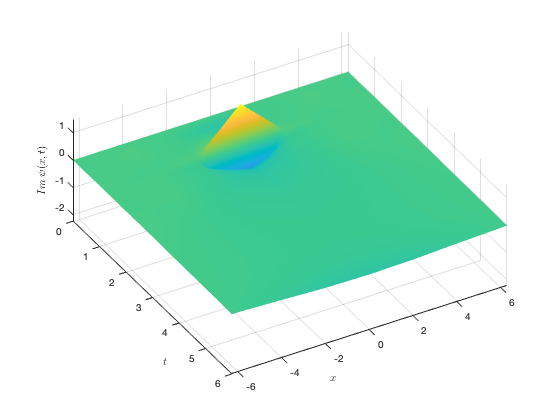
\includegraphics[scale=0.35]{with friction/b2imag.png}
        \end{center}  
    \end{multicols}
    \figurename{ 3.6 The real (left) and imaginary (right) parts of $\psi(x, t)$}
\end{enumerate}

\section{Twisted modes of the QNLS}
In this section we consider the \textit{sech-tanh} initial condition and propagate it according to \eqref{quad-NLS-lambda} --- the equation \eqref{quad-NLS-lambda} possesses two sets of solution known as the \textit{twisted} or \textit{sech-tanh} mode; the solutions are given as 
\begin{equation}\label{sech-tanh}
    u_{T}(x) = 2 \sech^2 (2x) \pm 2i \sech (2x) \tanh(2x).
\end{equation}
We simulate the two sets of solutions below.

\begin{enumerate}[label=(\alph*)]
    \item \textbf{Case 1}
    \newline
    
    Here we consider the first \textit{sech-mode}  $u_T(x) = 2 \sech^2 (2x) + 2i \sech (2x) \tanh(2x)$ as the initial condition and plugging this into \eqref{discrete-quad-NLS} yields the following results:
    \newpage
    \begin{enumerate}[label=(\roman*)]
    \item \textbf{Solution for $b=0$ and $\lambda=0$:}
    \begin{multicols}{2}
        \begin{center}
            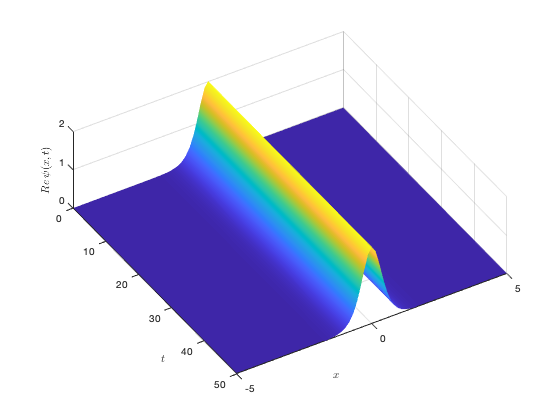
\includegraphics[scale=0.35]{twisted modes/lambda0real.png}
        \end{center}
        \begin{center}
            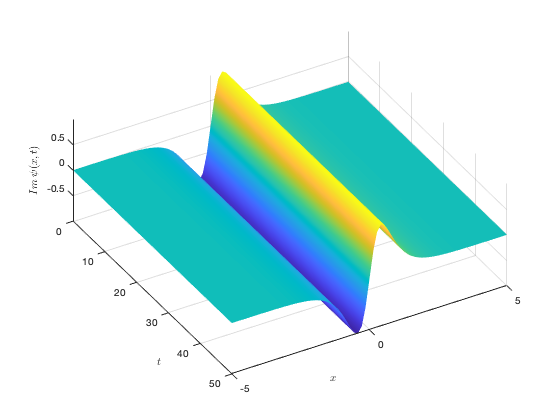
\includegraphics[scale=0.35]{twisted modes/lamda0imag.png}
        \end{center}
    \end{multicols}
    \figurename{ 4.1 The real (left) and imaginary (right) parts of $\psi(x, t)$}
    \newline
    
    \textbf{Solution for $b=0$, $\lambda=0.1$:}
    \begin{multicols}{2}
        \begin{center}
            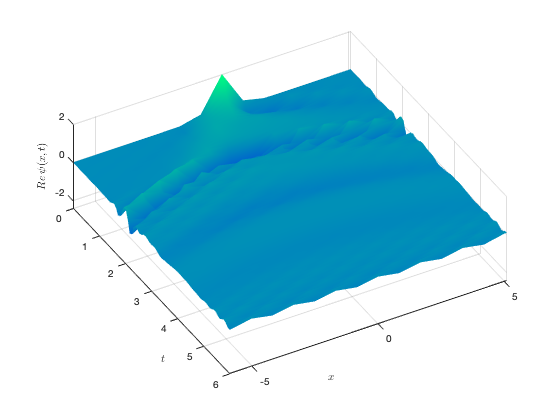
\includegraphics[scale=0.35]{twisted modes/lamda01real.png}
        \end{center}
        \begin{center}
            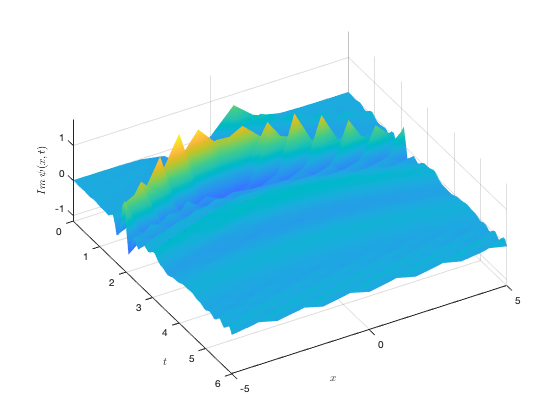
\includegraphics[scale=0.35]{twisted modes/lamda01imag.png}
        \end{center}
    \end{multicols}
    \figurename{ 4.2 The real (left) and imaginary (right) parts of $\psi(x, t)$}
    \end{enumerate}
    \newpage
    \item \textbf{Case 2}
    \newline
    
    We now consider $u_T(x) = 2 \sech^2 (2x) - 2i \sech (2x) \tanh(2x)$ as the initial condition. Plugging into \eqref{discrete-quad-NLS} yields the following results:
    
    \begin{enumerate}[label=(\roman*)]
        \item \textbf{Solution for $b=0$ and $\lambda=0$:}
        \begin{multicols}{2}
            \begin{center}
                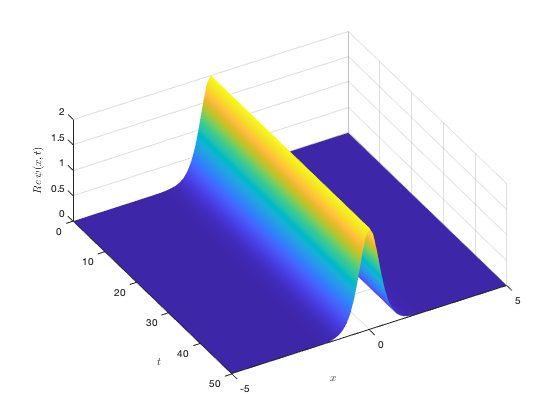
\includegraphics[scale=0.35]{twisted modes/lamda0minus_real.png}
            \end{center}
            \begin{center}
                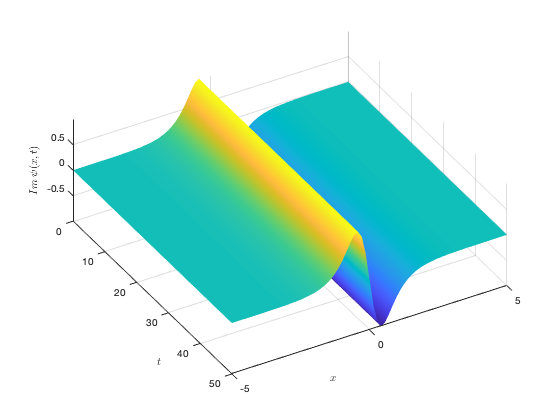
\includegraphics[scale=0.35]{twisted modes/lamda0minus_imag.png}
            \end{center}
        \end{multicols}
        \figurename{ 4.3 The real (left) and imaginary (right) parts of $\psi(x, t)$}
        
        \item \textbf{Solution for $b=0$ and $\lambda=0.1$:}
    \begin{multicols}{2}
        \begin{center}
            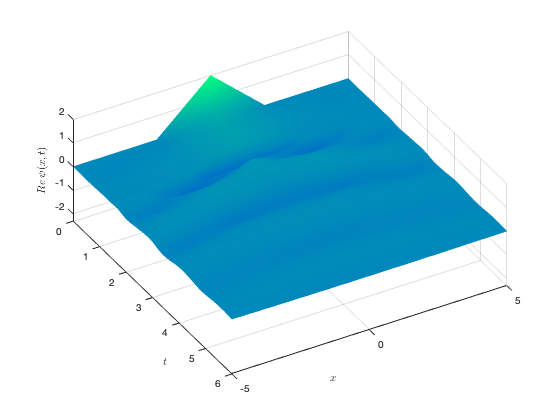
\includegraphics[scale=0.35]{twisted modes/lamda01minus_real.png}
        \end{center}
        \begin{center}
            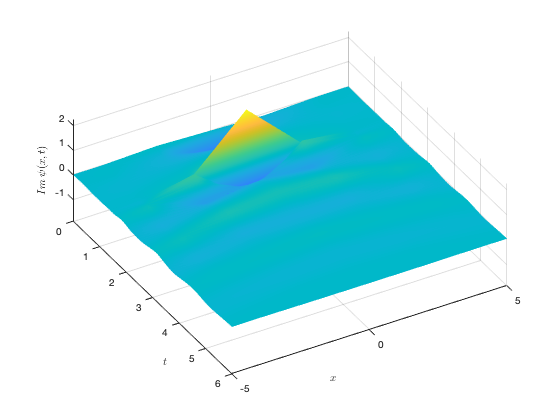
\includegraphics[scale=0.35]{twisted modes/lamda01minus_imag.png}
        \end{center}
    \end{multicols}
    \figurename{ 4.4 The real (left) and imaginary (right) parts of $\psi(x, t)$}
    \end{enumerate}
    
    
\end{enumerate}



\end{document}
